\chapter{Sorting Algorithms}

In this chapter we will look at some algorithms that sort an array of integers\footnote{The algorithms also work for other data types with linear order defined. However integer is selected for easier understanding.} of length \textit{n} in ascending order. We will look at how they work and analyze their efficiency (using time complexity). We will only focus on implementation using arrays.

To demonstrate different sorting algorithms, we would use this code right here as a template to verify whether the algorithms work:

\begin{lstlisting}
#include <iostream>
using namespace std;
int main(){
    int x[] = {3,1,4,1,5,9,2,6};
    
    //the sorting function accepts the array and the length of the array, this is common practice, as it is impossible to determine the length of the array in C/C++ when only the array is given.
    sort(x,8); //replace with name of the sorting function

    //print everything in x, with commas properly placed
    //check if the answer is 1,1,2,3,4,5,6,9
    cout << x[0];
    for(int i = 1; i < 8;  i++){
        cout << "," << x[i];
    }
    cout << endl;
}
\end{lstlisting}
\pagebreak
\section{Bubble sort}

Bubble sort swaps the places of two adjacent integers when it realizes they are out of order, until all integers are all sorted.

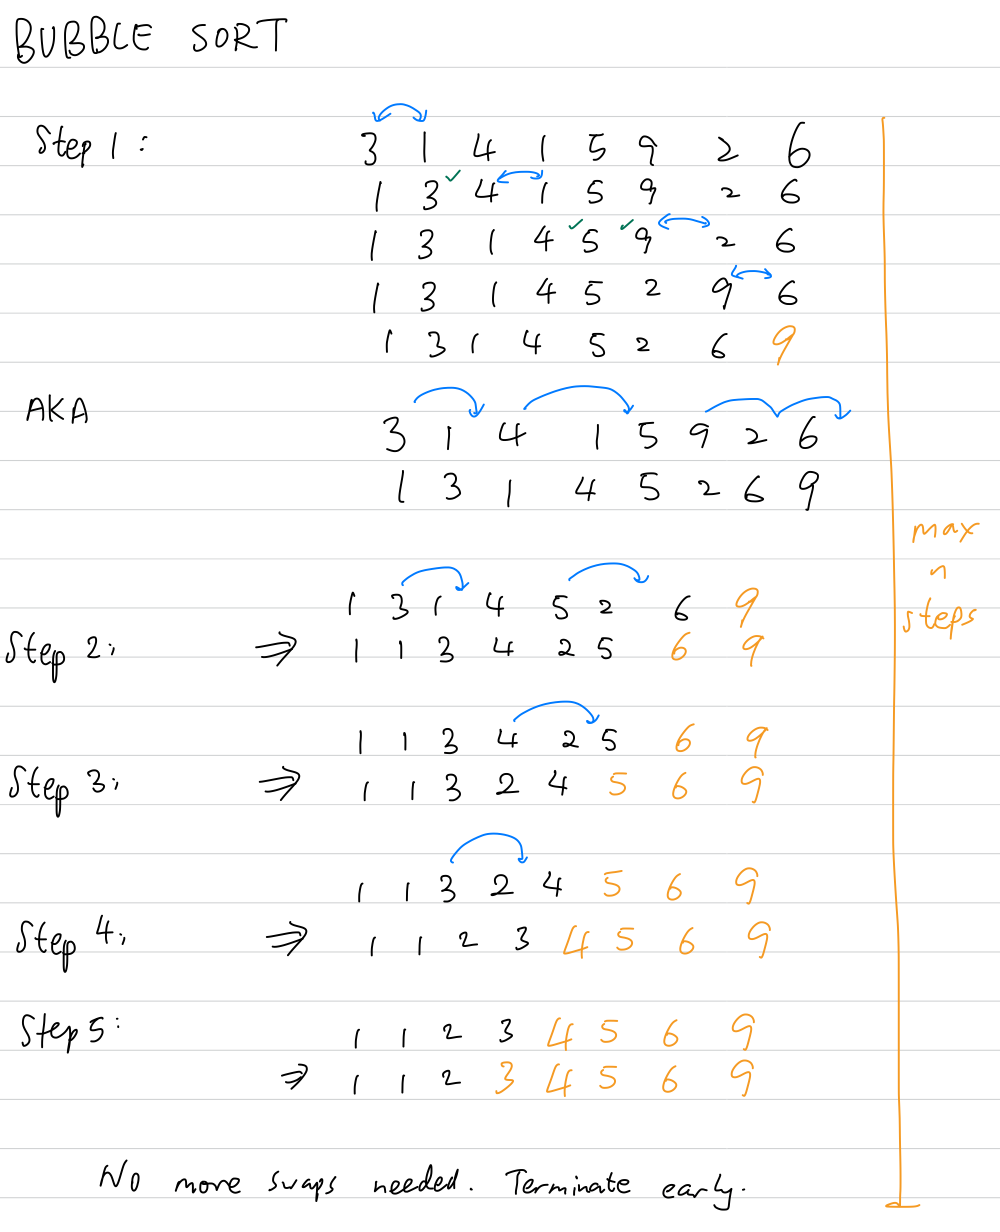
\includegraphics[width=15cm]{ch8-bubblesort.png}

\pagebreak

% Pseudocode:
% \begin{lstlisting}[language=Python,basicstyle=\rmfamily]
% bsort(x,n):
%     while(not sorted):
%         for j from 0 to n-1:
%             if x[j] > x[j+1]:
%                 swap(x[j],x[j+1]
% \end{lstlisting}

\pagebreak

At the \textit{i}th iteration of the outer loop, the last \textit{i} elements of the array are put at their sorted location. To guarantee the array is sorted, the inner loop is run \textit{n} times.


C++: (\textit{Exercise: Try to re-implement yourself.})
\begin{lstlisting}
void bsort(int x[], int n){
    for(int i = 0; i < n; i++){
        for(int j = 0; j < n-i-1; j++){ //the last i elements are sorted, no need to loop again
            if(x[j]>x[j+1]){
                int temp = x[j];
                x[j] = x[j+1];
                x[j+1] = temp;
            }
        } 
    }
}
\end{lstlisting}

Time complexity: $O(n^2)$ comparisons


There are \textit{n} steps, each step involves checking and swapping data from start to finish, taking time proportional to \textit{n} (in the worst case).

\pagebreak

\section{Selection sort}

Selection sort selects the minimum element and put it in front of the sorted array. Repeats until all elements are extracted.

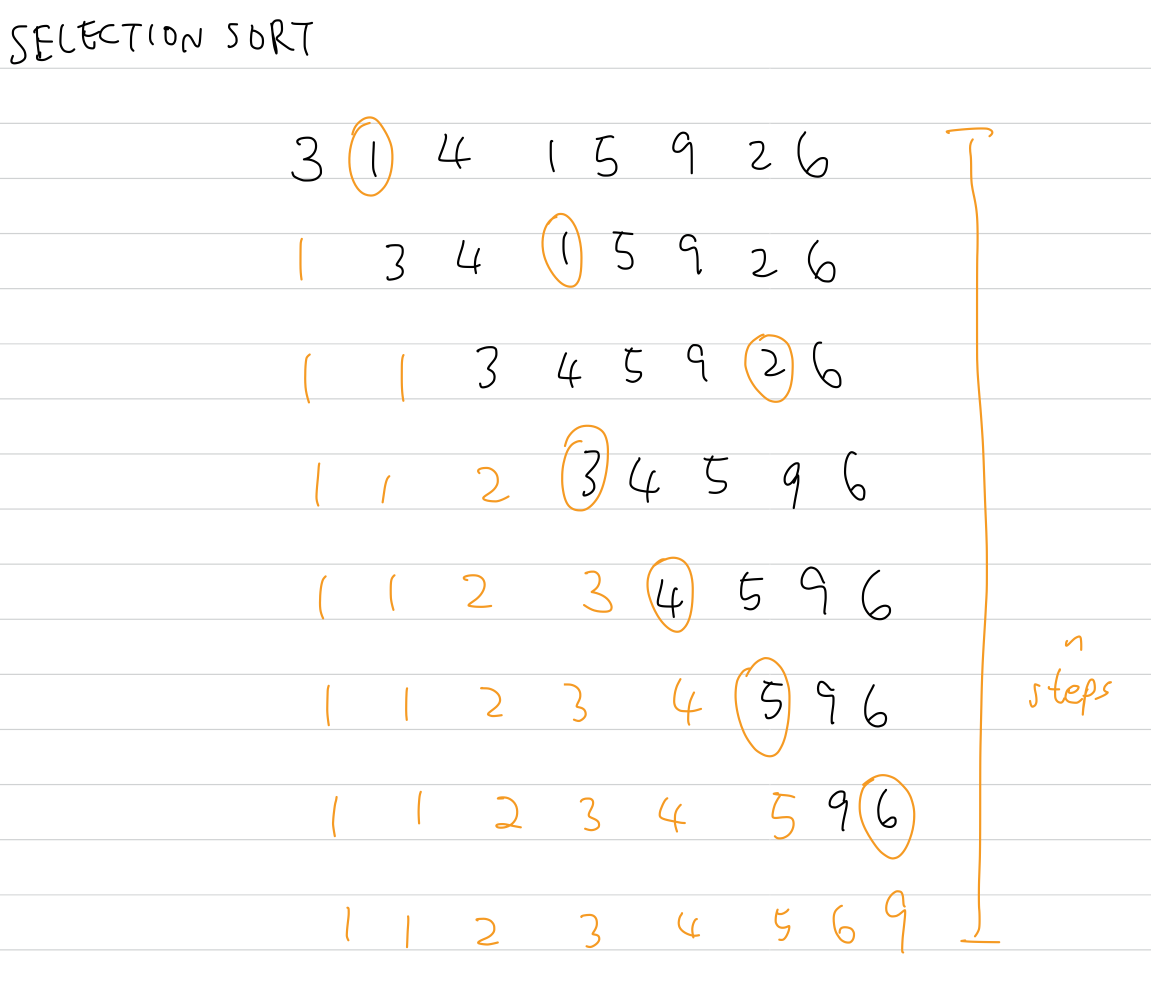
\includegraphics[width=16cm]{ch8-selectionsort.png}

\pagebreak

% Pseudocode:
% \begin{lstlisting}[language=Python,basicstyle=\rmfamily]
% ssort(x,n):
%     y = []
%     for each element in array x:
%         i = select-minimum(x) //get index of minimum element in x
%         y.append(x[i]) //add this element to the back of the newly created array
%         x.remove(i) //remove that minimum element from consideration
%     return y
% \end{lstlisting}

\pagebreak

C++: (\textit{Exercise: Try to re-implement yourself.})
\begin{lstlisting}
void ssort(int x[], int n){
    for(int i=0; i<n; i++){
    
        //find minimum value and its index in the array
        int minValue = x[i]; //Can we put 0 here instead?
        int minIndex = i;
        for(int j=i; j<n; j++){
            if(minValue > x[j]){
                minValue = x[j];
                minIndex = j;
            }
        }
        
        //swap x[i] with x[minIndex]
        x[minIndex] = x[i];
        x[i] = minValue;        
    }
}
\end{lstlisting}

Time complexity: $O(n^2)$ comparisons


There are \textit{n} steps, each step involves finding the minimum value, taking time proportional to \textit{n}.

\pagebreak

\section{Insertion sort}

Insertion sort assumes the leftmost element is a sorted array, then slowly adds elements in one by one, preserving the order of the sorted array.

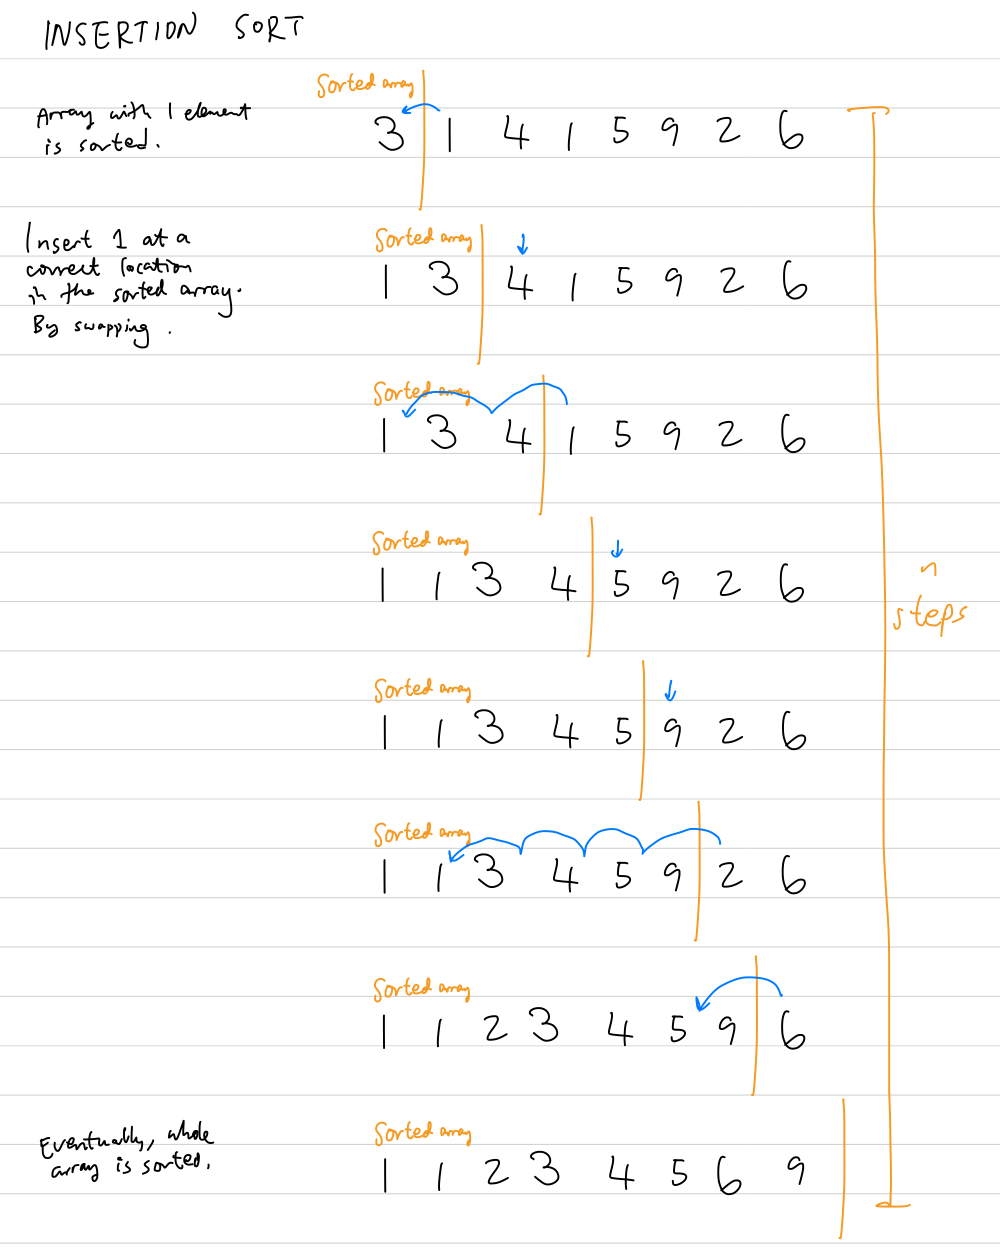
\includegraphics[width=15cm]{ch8-insertionsort.png}


% Pseudocode:
% \begin{lstlisting}[language=Python,basicstyle=\rmfamily]
% isort(x,n):
%     for i from 1 to n:
%         insert(x,i,x[i])

% insert(x,i,v):
%     j = i-1
%     while(j>0 and x[j] > v){
%         x[j+1] = x[j]
%         i--
%     }
%     x[j] = v
% \end{lstlisting}
% 
\pagebreak

C++: (\textit{Exercise: Try to re-implement yourself.})
\begin{lstlisting}
void isort(int x[], int n){
    for(int i=1; i<n; i++){
        int j = i-1;
        while(j>=0&&x[j] > x[j+1]){
            int temp = x[j];
            x[j] = x[j+1];
            x[j+1] = temp;
            j--;
        }
    }
}
\end{lstlisting}

Time complexity: $O(n^2)$ comparisons


There are \textit{n} steps, each step involves finding the correct location to insert the value concerned, taking time proportional to \textit{n}.

\pagebreak

\section{Merge sort}

\textit{Difficult topic}


Merge sort first splits the array repeatedly until all arrays are of length 1, where they are sorted without any actions. Then it merges back them two by two in order, eventually we get back the whole array in sorted order.

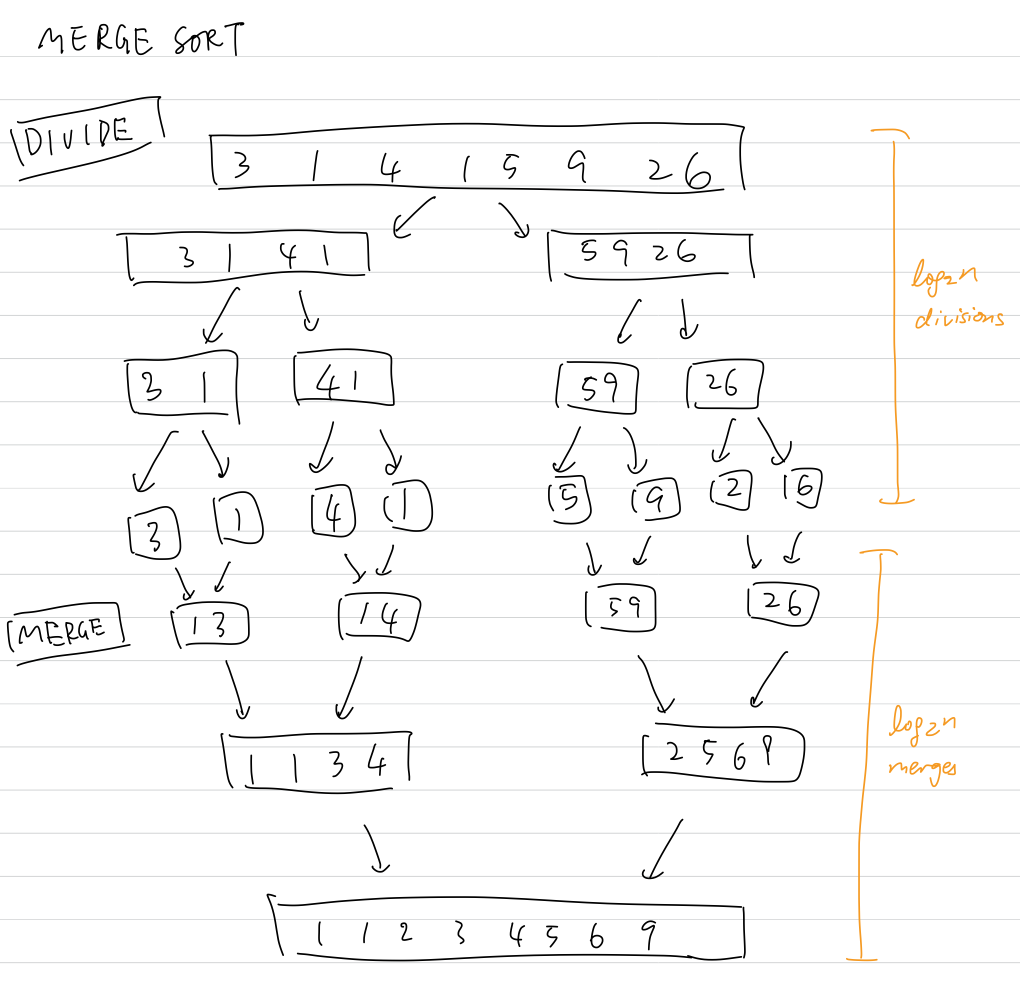
\includegraphics[width=15cm]{ch8-mergesort.png}

\pagebreak

% Pseudocode:
% \begin{lstlisting}[language=Haskell,basicstyle=\rmfamily]
% msort(x) = merge(msort(l),msort(r))
%     where l = first half of x, r = second half of x
% msort({}) = {}
% msort({a}) = {a} 

% merge(a,b)
%     | null a: b
%     | null b: a
%     | head a <= head b : [head a] ++ merge(tail a, b)
%     | else: [head b] ++ merge(a, tail b)
% \end{lstlisting}
% 

C++: (\textit{Exercise: Try to re-implement yourself.})

Call by \texttt{msort(x,0,8);}

\begin{lstlisting}
void merge(int x[], int a, int m, int b){
    //segment a: x[a..m)
    //segment b: x[m..b)

    //create array c that stores the result of the merge 
    int c[b-a];

    //store pointers of a,b,c to indicate the progress of the merge
    int ai = 0;
    int bi = 0; 
    int ci = 0;
    
    //perform the merge
    while(ai < m-a && bi < b-m){
        if(x[ai+a]<=x[bi+m]){
            c[ci] = x[ai+a];
            ci++;
            ai++;
        }else{
            c[ci] = x[bi+m];
            ci++;
            bi++;
        }
    }

    //one of the segments have completely used up, copy the remaining elements to the end of c
    while(ai < m-a){
        c[ci] = x[ai+a];
        ci++;
        ai++;
    }
    while(bi < b-m){
        c[ci] = x[bi+m];
        ci++;
        bi++;
    }

    //overwrite the data of the original segment with data in c
    for(int i=0;i<b-a;i++){
        x[i+a] = c[i];
    }
}

void msort(int x[], int start, int end){
    if(start+1>=end) return; //base case: the array is empty or with only 1 element
    int mid = (start+end)/2;
    msort(x,start,mid); //msort first half recursively [start..mid)
    msort(x,mid,end); //msort second half recursively [mid..end)
    merge(x,start,mid,end);
}
\end{lstlisting}

Time complexity: $O(n\log n)$ comparisons


There are $\log_2 n$ steps, each step involves function \textit{merge}, taking time proportional to \textit{n}.

\subsection*{A sprinkle of magic (OUT OF SCOPE)}

I know this piece of notes is probably too much for some of you, but as a Computer Science fanatic, I just have to give you something more to see. Well, you see the merge sort code took more than a page, but it can be much shorter in another programming language, Haskell. 

Here is the Haskell implementation:

\begin{lstlisting}[language=Haskell]
msort [] = []
msort [x] = [x]
msort xs = merge (msort ls) (msort rs)
    where (ls,rs) = halve xs

merge [] ys = ys
merge xs [] = xs
merge (x:xs) (y:ys) = if x <= y then x:merge xs (y:ys) else y:merge (x:xs) ys
    
halve xs = (take m xs, drop m xs)
    where m = (length xs) `div` 2

\end{lstlisting}

Of course you won't be able to understand the details of the code, but what I want you to know is that merge sort can be implemented with just 10 lines of code in some other languages. It is not necessarily one and a half page long.

\section{Quicksort}

\textit{Of less importance, difficult topic}


Don't have time to cover, there should be plenty of resources online on this topic.

% C++: (\textit{Exercise: Try to re-implement yourself.})

% Call by \texttt{qsort(x,0,8);}

% \begin{lstlisting}
% int partition(int x[], int l, int r){

%     //set the first element in x[l..r) to be the pivot
%     int p = x[l];
    
%     //refer to illustration on the maintenance of variables i and j
%     int i = l+1;
%     int j = r;
%     while(i<j){
%         if(x[i] < p){
%             i++;
%         }else{
%             j--;
%             int temp = x[i];
%             x[i] = x[j];
%             x[j] = temp;
%         }
%     }
    
%     //swap x[l] and x[i-1], so that the pivot is in the middle
%     x[l] = x[i-1];
%     x[i-1] = p;
    
%     //return location of the pivot
%     return i-1;
% }

% void qsort(int x[], int start, int end){
%     if(start+1 >= end) return; //base case: the array is empty or with only 1 element
%     int k = partition(x,start,end); 
    
%     //the array is now in three parts: 
%     //1. x[start..k) all have values < pivot 
%     //2. x[k] is the pivot
%     //3. x[k+1..end) all have values >= pivot
%     //we recursively sort the first and third parts
%     qsort(x,start,k);
%     qsort(x,k+1,end);
% }
% \end{lstlisting}
\section{Counting sort}

\textit{Of less importance}


Don't have time to cover, there should be plenty of resources online on this topic.

\section{Conclusion}

\begin{table}[h]
    \centering
    \begin{tabular}{|m{6em}|m{9em}|m{18em}|}
        \hline  
        \textbf{Sorting Algorithms} & 
        \multicolumn{2}{l|}{Goal: Sort elements in an array in ascending order}
        \\ \hline \hline
        
        Algorithm &
        Time Complexity & 
        Remarks
        \\ \hline \hline
        
        \makecell[lb]{Bubble sort \\ Selection sort \\ Insertion sort} &
        $O(n^2)$ &
        Only used on short arrays (seldom the case for programming competitions) because of their poor time complexity 
        \\ \hline
        
        \makecell[lb]{Merge sort \\ Quicksort} &
        $O(n\log n)$ &
        Good enough time complexity, without significant disadvantages. Hence they are used most often.
        \\ \hline
        
        Counting sort &
        $O(n)$ &
        Significant disadvantages, limited usage despite its fast time complexity, seldomly used. \tablefootnote{Know more about counting sort: \href{https://www.interviewcake.com/concept/java/counting-sort}{https://www.interviewcake.com/concept/java/counting-sort}}
        \\ \hline
    \end{tabular}
\end{table}

Merge sort and quicksort both have a time complexity of $O(n\log n)$, without significant disadvantages. Hence they are used most often. 


I hope you enjoyed the burst in knowledge, and if you are one of the contestants in the coming HKOI or other programming competitions, I also wish you all the best.